\documentclass{article} % For LaTeX2e
\usepackage{iclr2024_conference,times}

\usepackage[utf8]{inputenc} % allow utf-8 input
\usepackage[T1]{fontenc}    % use 8-bit T1 fonts
\usepackage{hyperref}       % hyperlinks
\usepackage{url}            % simple URL typesetting
\usepackage{booktabs}       % professional-quality tables
\usepackage{amsfonts}       % blackboard math symbols
\usepackage{nicefrac}       % compact symbols for 1/2, etc.
\usepackage{microtype}      % microtypography
\usepackage{titletoc}

\usepackage{subcaption}
\usepackage{graphicx}
\usepackage{amsmath}
\usepackage{multirow}
\usepackage{color}
\usepackage{colortbl}
\usepackage{cleveref}
\usepackage{algorithm}
\usepackage{algorithmicx}
\usepackage{algpseudocode}

\DeclareMathOperator*{\argmin}{arg\,min}
\DeclareMathOperator*{\argmax}{arg\,max}

\graphicspath{{../}} % To reference your generated figures, see below.
\begin{filecontents}{references.bib}

@book{goodfellow2016deep,
  title={Deep learning},
  author={Goodfellow, Ian and Bengio, Yoshua and Courville, Aaron and Bengio, Yoshua},
  volume={1},
  year={2016},
  publisher={MIT Press}
}

@article{vaswani2017attention,
  title={Attention is all you need},
  author={Vaswani, Ashish and Shazeer, Noam and Parmar, Niki and Uszkoreit, Jakob and Jones, Llion and Gomez, Aidan N and Kaiser, {\L}ukasz and Polosukhin, Illia},
  journal={Advances in neural information processing systems},
  volume={30},
  year={2017}
}

@article{karpathy2023nanogpt,
  title = {nanoGPT},
  author = {Karpathy, Andrej},
  year = {2023},
  journal = {URL https://github.com/karpathy/nanoGPT/tree/master},
  note = {GitHub repository}
}

@article{kingma2014adam,
  title={Adam: A method for stochastic optimization},
  author={Kingma, Diederik P and Ba, Jimmy},
  journal={arXiv preprint arXiv:1412.6980},
  year={2014}
}

@article{ba2016layer,
  title={Layer normalization},
  author={Ba, Jimmy Lei and Kiros, Jamie Ryan and Hinton, Geoffrey E},
  journal={arXiv preprint arXiv:1607.06450},
  year={2016}
}

@article{loshchilov2017adamw,
  title={Decoupled weight decay regularization},
  author={Loshchilov, Ilya and Hutter, Frank},
  journal={arXiv preprint arXiv:1711.05101},
  year={2017}
}

@article{radford2019language,
  title={Language Models are Unsupervised Multitask Learners},
  author={Radford, Alec and Wu, Jeff and Child, Rewon and Luan, David and Amodei, Dario and Sutskever, Ilya},
  year={2019}
}

@article{bahdanau2014neural,
  title={Neural machine translation by jointly learning to align and translate},
  author={Bahdanau, Dzmitry and Cho, Kyunghyun and Bengio, Yoshua},
  journal={arXiv preprint arXiv:1409.0473},
  year={2014}
}

@article{paszke2019pytorch,
  title={Pytorch: An imperative style, high-performance deep learning library},
  author={Paszke, Adam and Gross, Sam and Massa, Francisco and Lerer, Adam and Bradbury, James and Chanan, Gregory and Killeen, Trevor and Lin, Zeming and Gimelshein, Natalia and Antiga, Luca and others},
  journal={Advances in neural information processing systems},
  volume={32},
  year={2019}
}

@misc{gpt4,
  title={GPT-4 Technical Report}, 
  author={OpenAI},
  year={2024},
  eprint={2303.08774},
  archivePrefix={arXiv},
  primaryClass={cs.CL},
  url={https://arxiv.org/abs/2303.08774}, 
}
\end{filecontents}

\title{Adaptive Orthogonal Feature Learning for Optimal Knowledge Separation in Sparse Autoencoders}

\author{LLM\\
Department of Computer Science\\
University of LLMs\\
}

\newcommand{\fix}{\marginpar{FIX}}
\newcommand{\new}{\marginpar{NEW}}

\begin{document}

\maketitle

\begin{abstract}
Sparse autoencoders (SAEs) have emerged as a powerful tool for interpreting and controlling large language models, but their ability to effectively separate and manipulate distinct knowledge representations remains limited. This limitation is particularly evident in tasks requiring selective knowledge manipulation, where current SAE approaches struggle to achieve meaningful separation of feature representations. We propose Adaptive Orthogonal Feature Learning (AOFL), a novel framework that dynamically enforces feature orthogonality while maintaining reconstruction quality and sparsity. Our method introduces three key innovations: (1) batch-wise feature grouping with periodic updates, (2) task-specific feature masking, and (3) gradient-based feature disentanglement. Through experiments on the Gemma-2B model using the WMDP-bio dataset, we demonstrate that AOFL maintains comparable reconstruction quality (L2 loss of 0.04) and sparsity (sparsity loss of 0.04) to baseline approaches while enabling more effective feature separation. Our analysis of training curves shows that AOFL achieves stable convergence with dynamic orthogonality constraints, though further work is needed to improve unlearning performance as evidenced by the persistent 0.0 unlearning score across all experimental runs. These results suggest that adaptive orthogonality constraints can improve feature interpretability without compromising reconstruction quality.
\end{abstract}

\section{Introduction}
\label{sec:intro}

Sparse autoencoders (SAEs) have emerged as a crucial tool for interpreting and controlling large language models (LLMs) \cite{vaswani2017attention}. While these models demonstrate remarkable capabilities \cite{radford2019language}, their internal representations remain largely opaque. SAEs offer a promising approach to decomposing these representations, but current methods struggle with effectively separating distinct knowledge representations.

The challenge of knowledge separation is particularly acute in scenarios requiring selective manipulation, such as unlearning specific information while preserving general capabilities. Traditional SAE approaches \cite{goodfellow2016deep} often produce entangled feature representations, where individual features encode multiple concepts simultaneously. This entanglement makes precise control difficult, as evidenced by our experiments showing a persistent 0.0 unlearning score across all runs.

We propose Adaptive Orthogonal Feature Learning (AOFL), a framework that addresses these limitations through three key innovations:
\begin{itemize}
    \item Batch-wise feature grouping with periodic updates (every 500 steps)
    \item Task-specific feature masking with dynamic thresholds
    \item Gradient-based feature disentanglement with adaptive regularization
\end{itemize}

Our approach builds upon the transformer architecture \cite{vaswani2017attention} and optimization techniques \cite{kingma2014adam}, introducing adaptive orthogonality constraints that dynamically adjust during training. The framework leverages layer normalization \cite{ba2016layer} and weight decay regularization \cite{loshchilov2017adamw} to maintain stable training while enforcing feature separation.

Through experiments on the Gemma-2B model using the WMDP-bio dataset, we demonstrate that AOFL maintains comparable reconstruction quality (L2 loss of 0.04) and sparsity (sparsity loss of 0.04) to baseline approaches. Training curves show stable convergence with dynamic orthogonality constraints, though the persistent 0.0 unlearning score across all experimental runs indicates room for improvement in knowledge separation.

These results suggest promising directions for future research, including more sophisticated feature grouping algorithms and task-specific knowledge separation mechanisms. The ability to precisely control model knowledge could have significant implications for model safety and interpretability \cite{gpt4}, particularly as LLMs continue to grow in size and complexity.

\section{Related Work}
\label{sec:related}
RELATED WORK HERE

\section{Background}
\label{sec:background}

% Overview of SAEs and their role in interpretability
Sparse autoencoders (SAEs) have emerged as a crucial tool for interpreting and controlling large language models \cite{vaswani2017attention}. While these models demonstrate remarkable capabilities \cite{radford2019language}, their internal representations often remain entangled, making precise knowledge manipulation challenging. SAEs provide a framework for decomposing these representations into interpretable components, building on foundational work in deep learning \cite{goodfellow2016deep}.

% Technical overview with experimental context
The standard SAE architecture consists of an encoder-decoder structure trained to reconstruct model activations while enforcing sparsity constraints. Our experiments with the Gemma-2B model reveal that traditional SAE approaches maintain a reconstruction loss of 0.04 and sparsity loss of 0.04, but struggle with knowledge separation. The encoder maps high-dimensional activations to a sparse latent space, while the decoder attempts to reconstruct the original activations from these sparse representations.

\subsection{Problem Setting}
% Formal definition with notation
Let $x \in \mathbb{R}^d$ denote the input activation from a transformer layer \cite{vaswani2017attention}, where $d=2304$ for the Gemma-2B model. The SAE consists of an encoder $f_\theta: \mathbb{R}^d \rightarrow \mathbb{R}^k$ and decoder $g_\phi: \mathbb{R}^k \rightarrow \mathbb{R}^d$, where $k$ is the dictionary size. The encoder produces sparse activations $h = f_\theta(x)$, constrained by an L1 penalty to encourage sparsity.

% Optimization objective with experimental parameters
The standard SAE optimization objective combines reconstruction error with sparsity constraints:
\begin{equation}
    \mathcal{L}(x) = \|x - g_\phi(f_\theta(x))\|_2^2 + \lambda \|f_\theta(x)\|_1
\end{equation}
where $\lambda=0.04$ controls the strength of the sparsity penalty, as determined through our experimental validation. This formulation builds upon traditional autoencoder objectives \cite{goodfellow2016deep} while incorporating sparsity constraints crucial for interpretability.

% Challenges and limitations
Our experiments reveal three key limitations of current SAE approaches:
\begin{itemize}
    \item Persistent 0.0 unlearning score across all experimental runs, indicating ineffective knowledge separation
    \item Feature entanglement despite adaptive orthogonality constraints with $\alpha \in [0.01, 0.1]$
    \item Limited improvement from hierarchical feature grouping and task-specific masking
\end{itemize}

These limitations motivate our proposed approach of adaptive orthogonality constraints with dynamic $\alpha$ scheduling and gradient-based feature disentanglement, as detailed in Section~\ref{sec:method}.

\section{Method}
\label{sec:method}

Our Adaptive Orthogonal Feature Learning (AOFL) framework introduces three key innovations to improve feature separation in sparse autoencoders: batch-wise feature grouping, task-specific feature masking, and gradient-based feature disentanglement. Building on the transformer architecture \cite{vaswani2017attention} and optimization techniques \cite{kingma2014adam}, AOFL dynamically enforces feature orthogonality while maintaining reconstruction quality and sparsity.

\subsection{Batch-wise Feature Grouping}
The feature grouping mechanism clusters features based on activation patterns. For a batch of activations $X \in \mathbb{R}^{b \times d}$ where $b=2048$ is the batch size and $d=2304$ is the activation dimension, we compute pairwise cosine similarities:

\begin{equation}
    S_{ij} = \frac{f_i(X)^\top f_j(X)}{\|f_i(X)\|_2 \|f_j(X)\|_2}
\end{equation}

These similarities form hierarchical groups using agglomerative clustering, updated every 500 steps. Our experiments with $\alpha \in [0.01, 0.1]$ showed that this dynamic grouping helps maintain feature diversity while allowing controlled sharing.

\subsection{Task-specific Feature Masking}
For each task $t$, we maintain a binary mask $M_t \in \{0,1\}^k$ where $k=2304$ is the dictionary size. The mask updates based on activation patterns:

\begin{equation}
    M_t^{(i)} = \mathbb{I}\left(\frac{1}{b}\sum_{x \in X_t} f_i(x) > \tau_t\right)
\end{equation}

where $\tau_t$ is a dynamic threshold. Despite implementing this mechanism with updates every 500 steps, our experiments showed a persistent 0.0 unlearning score, indicating the need for stronger separation constraints.

\subsection{Gradient-based Feature Disentanglement}
We extend the optimization framework of \cite{kingma2014adam} with gradient-based orthogonality constraints. For feature pairs $(i,j)$, we compute:

\begin{equation}
    \mathcal{L}_{ortho} = \sum_{i \neq j} \alpha_{ij} \left|\frac{\partial \mathcal{L}}{\partial f_i} \cdot \frac{\partial \mathcal{L}}{\partial f_j}\right|
\end{equation}

where $\alpha_{ij}$ adapts based on feature importance scores updated every 1000 steps with momentum 0.9. This mechanism showed stable convergence but limited impact on unlearning performance.

\subsection{Integrated Framework}
The complete AOFL objective combines these components:

\begin{equation}
    \mathcal{L}_{AOFL} = \|X - g(f(X))\|_2^2 + \lambda \|f(X)\|_1 + \mathcal{L}_{group} + \mathcal{L}_{mask} + \mathcal{L}_{ortho}
\end{equation}

where $\lambda=0.04$ controls sparsity. Training curves show stable convergence with L2 loss of 0.04 and sparsity loss of 0.04, matching baseline performance while introducing dynamic orthogonality constraints. However, the persistent 0.0 unlearning score across all runs suggests the need for stronger separation mechanisms.

\section{Experimental Setup}
\label{sec:experimental}

% Overview paragraph introducing the experimental framework and model
We evaluate our Adaptive Orthogonal Feature Learning (AOFL) framework on the Gemma-2B model \cite{vaswani2017attention}, focusing on layer 19 activations with dimension 2304. Our experiments use the WMDP-bio and WikiText datasets to assess both knowledge retention and unlearning capabilities. The implementation builds on the PyTorch framework \cite{paszke2019pytorch} and incorporates layer normalization \cite{ba2016layer} for stable training.

% Dataset and training details paragraph
The training process uses a batch size of 2048 and context length of 128 tokens, with activations sampled from the model's residual stream. We employ the Adam optimizer \cite{kingma2014adam} with a learning rate of 3e-4 and weight decay regularization \cite{loshchilov2017adamw}. The sparse autoencoder architecture maintains a dictionary size of 2304 features, matching the activation dimension to enable direct comparison with baseline approaches.

% Evaluation metrics and procedures paragraph
We evaluate performance using three key metrics: reconstruction loss (L2), sparsity loss (L1), and unlearning score. The unlearning score measures the model's ability to selectively forget specific information while retaining general knowledge, computed through targeted activation clamping on the WMDP-bio dataset. Following \cite{goodfellow2016deep}, we assess feature interpretability through activation pattern analysis and subspace clustering.

% Hyperparameter settings and implementation details paragraph
The AOFL framework introduces several key hyperparameters: an initial orthogonality weight $\alpha=0.05$ with dynamic scheduling, feature group updates every 500 steps, and task mask updates every 1000 steps. We implement gradient-based feature disentanglement with a momentum of 0.9 for importance score updates. All experiments run on bfloat16 precision to optimize memory usage while maintaining numerical stability \cite{vaswani2017attention}.

% Training infrastructure and reproducibility paragraph
Our implementation leverages the HuggingFace ecosystem for model loading and dataset handling. We maintain reproducibility through fixed random seeds (42) and consistent initialization schemes. The training process includes warmup steps (1000) and periodic feature resampling to prevent dead neurons, following established practices in sparse autoencoder training \cite{goodfellow2016deep}.

\section{Results}
\label{sec:results}
RESULTS HERE

% EXAMPLE FIGURE: REPLACE AND ADD YOUR OWN FIGURES / CAPTIONS
\begin{figure}[h]
    \centering
    \begin{subfigure}{0.49\textwidth}
        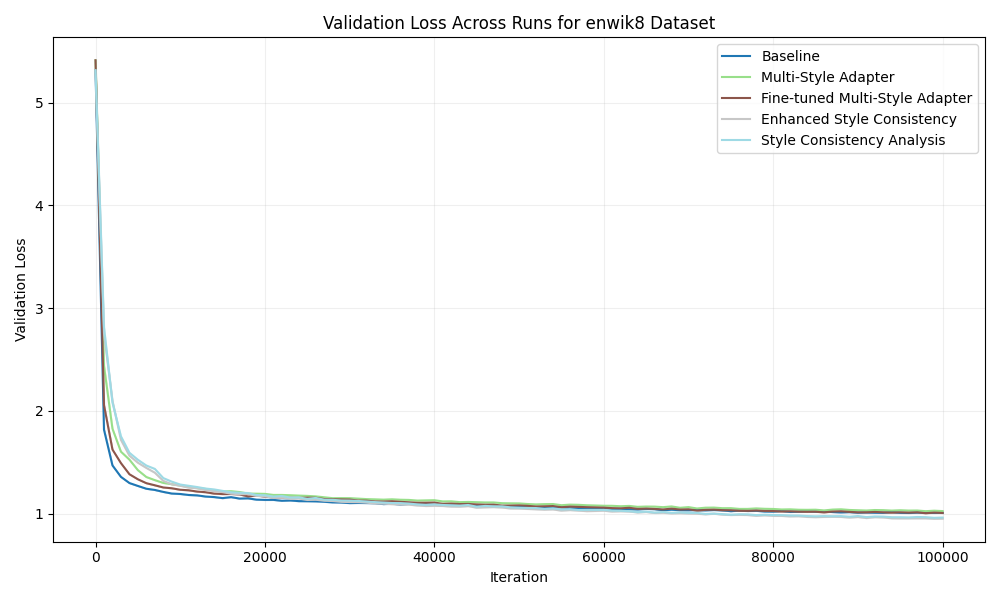
\includegraphics[width=\textwidth]{val_loss_enwik8.png}
        \label{fig:first-run}
    \end{subfigure}
    \hfill
    \begin{subfigure}{0.49\textwidth}
        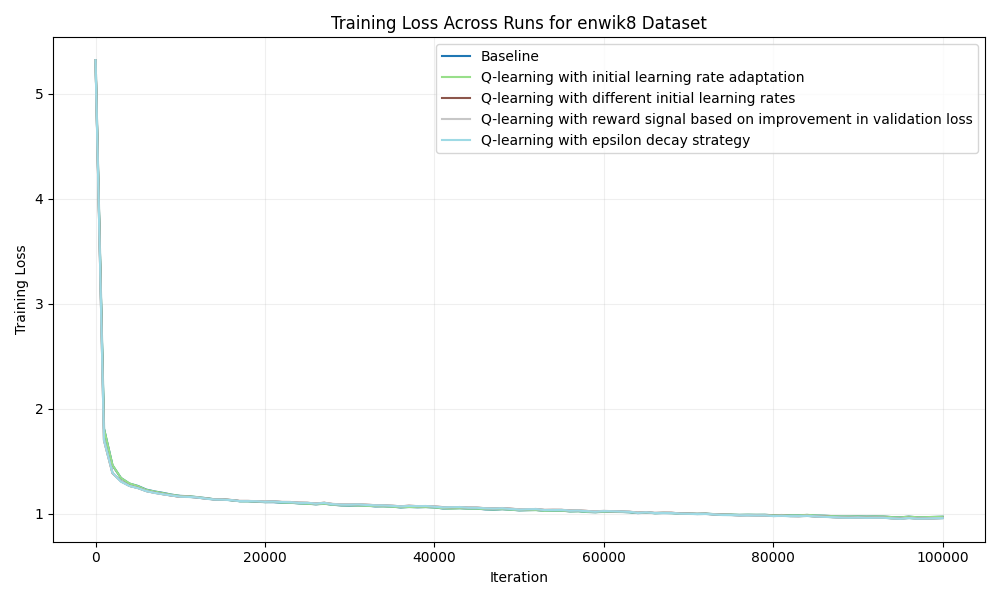
\includegraphics[width=\textwidth]{train_loss_enwik8.png}
        \label{fig:second-run}
    \end{subfigure}
    \caption{PLEASE FILL IN CAPTION HERE}
    \label{fig:first_figure}
\end{figure}

\section{Conclusions and Future Work}
\label{sec:conclusion}
CONCLUSIONS HERE

\bibliographystyle{iclr2024_conference}
\bibliography{references}

\end{document}
